\documentclass{beamer}
%\usepackage[margin=1in]{geometry}
\usepackage{amsthm,amsmath,amsfonts,hyperref,graphicx,color,multicol}
\usepackage{enumitem,tikz}

%%%%%%%%%%
%Beamer Template Customization
%%%%%%%%%%
\setbeamertemplate{navigation symbols}{}
\setbeamertemplate{theorems}[ams style]
\setbeamertemplate{blocks}[rounded]

\definecolor{Blu}{RGB}{43,62,133} % UWEC Blue
\setbeamercolor{structure}{fg=Blu} % Titles

%Unnumbered footnotes:
\newcommand{\blfootnote}[1]{%
	\begingroup
	\renewcommand\thefootnote{}\footnote{#1}%
	\addtocounter{footnote}{-1}%
	\endgroup
}


%%%%%%%%%%
%Custom Commands
%%%%%%%%%%
\newcommand{\R}{\mathbb{R}}
\newcommand{\veca}{\vec{a}}
\newcommand{\vecb}{\vec{b}}
\newcommand{\vece}{\vec{e}}
\newcommand{\vecu}{\vec{u}}
\newcommand{\vecv}{\vec{v}}
\newcommand{\vecw}{\vec{w}}
\newcommand{\vecx}{\vec{x}}
\newcommand{\zerovector}{\vec{0}}

\newcommand{\ds}{\displaystyle}

\newcommand{\fn}{\insertframenumber}

\newcommand{\rank}{\operatorname{rank}}
\newcommand{\adj}{\operatorname{adj}}

\newcommand{\blank}[1]{\underline{\hspace*{#1}}}


%%%%%%%%%%
%Custom Theorem Environments
%%%%%%%%%%
\theoremstyle{definition}
\newtheorem{exercise}{Exercise}
\newtheorem{question}[exercise]{Question}
\newtheorem*{defn}{Definition}
\newtheorem*{exa}{Example}
\newtheorem*{disc}{Group Discussion}
\newtheorem*{nb}{Note}
\newtheorem*{recall}{Recall}
\renewcommand{\emph}[1]{{\color{blue}\texttt{#1}}}

\definecolor{Gold}{RGB}{237, 172, 26}
%Statement block
\newenvironment{statementblock}[1]{%
	\setbeamercolor{block body}{bg=Gold!20}
	\setbeamercolor{block title}{bg=Gold}
	\begin{block}{\textbf{#1.}}}{\end{block}}





\begin{document}
	\title{Math 324: Linear Algebra}
	\subtitle{Section 3.4: Applications of Determinants}
	\author{Mckenzie West}
	\date{Last Updated: \today}
\begin{frame}
\maketitle
\end{frame}

\begin{frame}{\insertframenumber}
	\begin{block}{\textbf{Last Time.}}
	\begin{itemize}[label=--]
		\item More Properties of Determinants
		\item The Adjoin of a Matrix
		\item Cramer's Rule
	\end{itemize}
	\end{block}
	\begin{block}{\textbf{Today.}}
		\begin{itemize}[label=--]
			\item Areas and Volumes
			\item Lines and Planes
			\item Cross Products
		\end{itemize}
	\end{block}
\end{frame}

\begin{frame}{\fn}
	\begin{block}{\textbf{Area of a Parallelogram}}
			The area of the parallelogram defined by $(a,b)$ and $(c,d)$ is	
			\[\text{Area}=\begin{Vmatrix}a&b\\c&d\end{Vmatrix},\]
			where $\begin{Vmatrix}A\end{Vmatrix}$ denotes the absolute value of the determinant.
			\begin{center}
			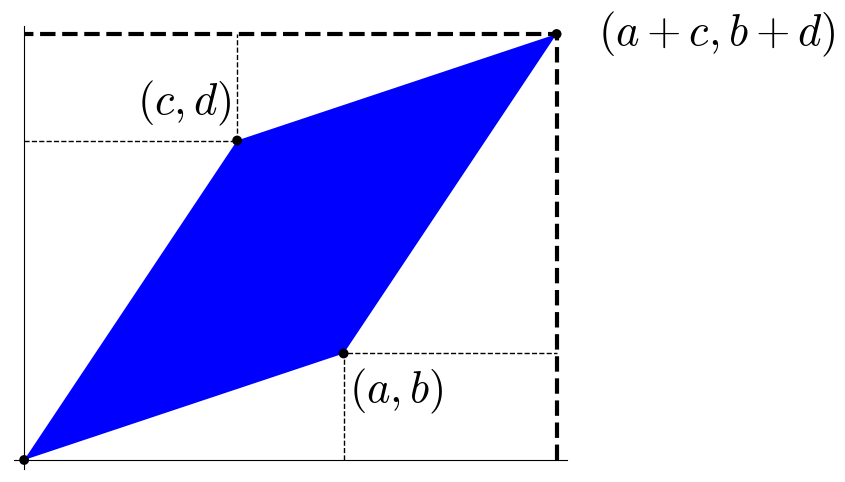
\includegraphics[width=1.5in]{images/parallelogram}
			\end{center}
	\end{block}
	\begin{exercise}
		Geometrically verify this formula using areas of rectangles and triangles.
		
		Then find the area of the parallelogram defined by $(3,1)$ and $(2,3)$.
	\end{exercise}
\end{frame}

\begin{frame}{\fn}
	\begin{block}{\textbf{Area of a Triangle in the $xy$-Plane}}
		\begin{minipage}{.65\textwidth}
			The area of the triangle with vertices	\[(x_1,y_1), (x_2,y_2), \text{ and } (x_3,y_3)\] can be calculated using
		
			\[\text{Area}=\frac{1}{2}\begin{Vmatrix}x_1&y_1&1\\x_2&y_2&1\\x_3&y_3&1\end{Vmatrix}.\]
		\end{minipage}
		\begin{minipage}{.3\textwidth}
			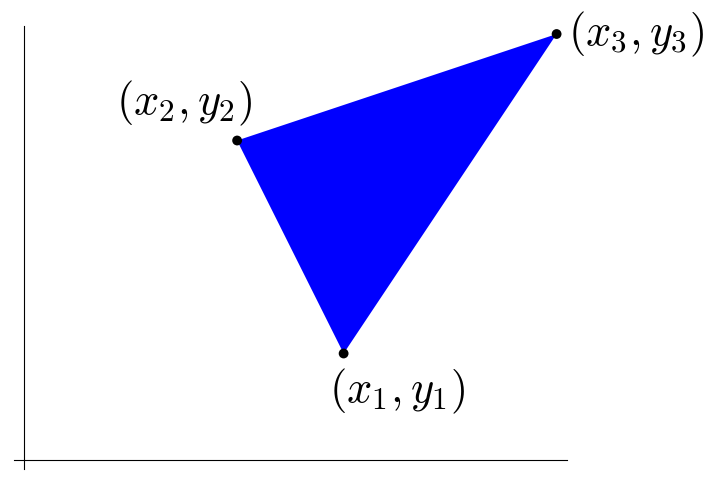
\includegraphics[width=\textwidth]{images/triangle}
		\end{minipage}
	\end{block}
	\begin{exercise}
		Find the area of the triangle with vertices $(0,1),(3,2)$, and $(5,7)$.
	\end{exercise}
\end{frame}

\begin{frame}{\fn}
	\begin{nb}
		If three points are \emph{co-linear}--meaning they all lie on the same line--then they will form a triangle with zero area.  
	\end{nb}
	\begin{exercise} Which of the following sets of points are co-linear?  Use the area formula from the last slide.
		\begin{enumerate}[label=(\alph*)]
			\item $(0,1),(2,5),(4,-2)$
			\item $(-2,-7),(0,-1),(3,8)$
			\item $(2,1),(2,2),(2,3)$
		\end{enumerate}
	\end{exercise}
\end{frame}

\begin{frame}{\fn}
	\begin{nb}
		Given two points, any other point $(x,y)$ that is co-linear to these two will produce a triangle of zero area.
	\end{nb}
	\begin{block}{\textbf{Two-Point Form of the Equation of a Line}}
		An equation for the line passing through the points $(x_1,y_1)$ and $(x_2,y_2)$ is given by	
			\[0=\begin{vmatrix}x&y&1\\x_1&y_1&1\\x_2&y_2&1\end{vmatrix}.\]
	\end{block}
	\begin{exercise}
		Use the determinant formula to find an equation for the line passing through the points
			\begin{enumerate}[label=(\alph*)]
				\item $(-3,2)$ and $(1,5)$
				\item $(1,1)$ and $(-10,1)$
			\end{enumerate}
	\end{exercise}
\end{frame}
\begin{frame}{\fn}
	\begin{exercise}
		Use the determinant formula to verify the point slope formula of the line passing through the points $(x_1,y_1)$ and $(x_2,y_2)$:
			\[y-y_1=m(x-x_1)\]
		where $\ds m=\frac{y_2-y_1}{x_2-x_1}$.
	\end{exercise}
\end{frame}

\begin{frame}{\fn}
	\begin{block}{\textbf{Brain Break.}}
		If teleportation were possible, what would be the first place you’d teleport to?
		\begin{center}
			
\includegraphics[width=1in]{images/teleporter}
		\end{center}
	\end{block}
\end{frame}

\begin{frame}{\fn}
	\begin{block}{\textbf{Volume of a Tetrahedron.}}
		The volume of the tetrahedron with vertices $(x_1,y_1,z_1)$, $(x_2,y_2,z_2)$, $(x_3,y_3,z_3)$, and $(x_4,y_4,z_4)$ is given by
			\[\text{Volume}=\frac{1}{6}\begin{Vmatrix}x_1&y_1&z_1&1\\x_2&y_2&z_2&1\\x_3&y_3&z_3&1\\x_4&y_4&z_4&1\end{Vmatrix}.\]
	\end{block}
	\begin{exercise}
		\begin{minipage}{.65\textwidth}Find the volume of the Tetrahedron with vertices $(1,0,1)$, $(1,3,2)$, $(4,7,1)$, and $(-1,0,0)$.\end{minipage}
		\begin{minipage}{.3\textwidth}
				\begin{center}
				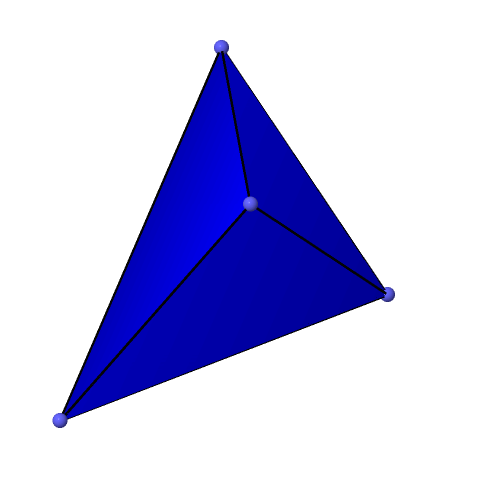
\includegraphics[width=1in]{images/tetrahedron}
			\end{center}
		\end{minipage}
	\end{exercise}
\end{frame}

\begin{frame}{\fn}
	\begin{nb}
		If four points are \emph{co-planar}--meaning they all lie on the same plane--then they will form a tetrahedron with zero area.  
	\end{nb}
	\begin{exercise} Which of the following sets of points are co-planar?  Use the volume formula from the last slide.
		\begin{enumerate}[label=(\alph*)]
			\item $(-2, -2, 1)$, $(1, -3, -1)$, $(-1, -2, -3)$, $(-2, -3, 3)$
			\item $(-2, 3, 2)$, $(0, -2, 1)$, $(3, 3, -3)$, $(3, -2, -2)$
			\item $(-3, -1, 1)$, $(1, 3, 1)$, $(2, 2, 2)$, $(-1, -1, 2)$
		\end{enumerate}
	\end{exercise}
\end{frame}

\begin{frame}{\fn}
	\begin{nb}
		Given three points in 3-d space, any other point $(x,y,z)$ that is co-planar to these three will produce a tetrahedron of zero volume.
	\end{nb}
	\begin{block}{\textbf{Three-Point Form of the Equation of a Plane}}
		An equation for the line passing through the points $(x_1,y_1,z_1)$, $(x_2,y_2,z_2)$, and $(x_3,y_3,z_3)$ is given by	
		\[0=\begin{vmatrix}x&y&z&1\\x_1&y_1&z_1&1\\x_2&y_2&z_2&1\\x_3&y_3&z_3&1\end{vmatrix}.\]
	\end{block}
	\begin{exercise}
		Use the determinant formula to find an equation for the plane passing through the points $(3, -3, 3)$, $(-1, 0, -2)$, and $(-2, -1, -2)$
	\end{exercise}
\end{frame}
\begin{frame}{\fn}
	\begin{exercise}
		The following three points lie on a single line in 3-d:
		$(-1, 0, -2)$, $(-2, -1, -2)$, $(-3, -2, -2)$.  What happens when you try to find the plane that contains the three points?
		\vskip -.25in
			\begin{center}
				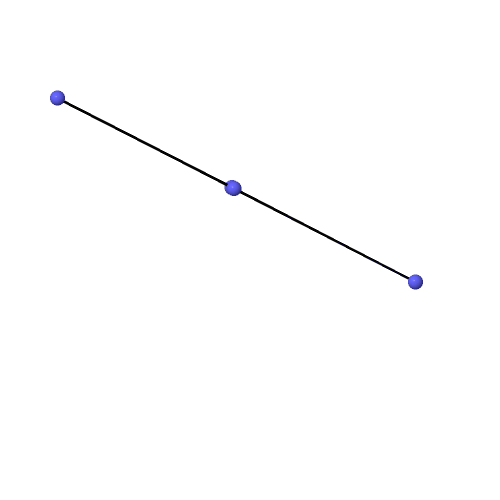
\includegraphics[width=2in]{images/line}
			\end{center}
		\vskip -.5in
		A line in 3-d requires two linear equations: $a_1x+b_1y+c_1z=d_1$ and $a_2x+b_2y+c_2z=d_1$.  Find an equation for the line containing these three points.
	\end{exercise}
\end{frame}

%\begin{frame}{\fn}
%	\begin{defn}
%		Let $\vece_1=\begin{bmatrix}1\\0\\0\end{bmatrix}$, $\vece_2=\begin{bmatrix}0\\1\\0\end{bmatrix}$, and $\vece_3=\begin{bmatrix}0\\0\\1\end{bmatrix}$ be the \emph{standard basis for $\R^3$}.  That is, every $3\times 1$ column matrices can easily be written as a linear combination of $\vece_1,\vece_2$, and $\vece_3$.
%		
%		The \emph{cross product} of two $3\times 1$ column matrices, $\vecu=\begin{bmatrix}u_1\\u_2\\u_3\end{bmatrix}$ and $\vecv=\begin{bmatrix}v_1\\v_2\\v_3\end{bmatrix}$, is defined to be the $3\times 1$ column matrices given by:
%		
%		\[\vecu\times\vecv=\begin{vmatrix}
%		\vece_1&u_1&v_1\\\vece_2&u_2&v_2\\\vece_3&u_3&v_3
%		\end{vmatrix}~.\]
%	\end{defn}
%\end{frame}
%\begin{frame}{\fn}
%	\begin{exercise}
%		Use the determinant formula to find
%			\[\begin{bmatrix}3\\-2\\5\end{bmatrix}\times\begin{bmatrix}0\\2\\0\end{bmatrix}.\]
%	\end{exercise}
%	\begin{exercise}
%		Write $\begin{bmatrix}u_1\\u_2\\u_3\end{bmatrix}\times\begin{bmatrix}v_1\\v_2\\v_3\end{bmatrix}$ as a $3\times 1$ column matrix.
%	\end{exercise}
%\end{frame}
%\begin{frame}{\fn}
%	\begin{exercise}
%		Use properties of the determinant to show:
%				\begin{enumerate}[label=(\alph*)]
%				\item $\vecv\times \vecu=-(\vecu\times \vecv)$
%				\item $\vecu\times \zerovector=\zerovector$
%				\item $\vecu\times\vecu=\zerovector$
%				\item $\vecu\times (k\vecv)=k(\vecu\times\vecv)$
%				\item $\vecu\times(\vecv+\vecw)=(\vecu\times \vecv)+(\vecu\times \vecw)$
%				\item $\vecu^T(\vecv\times\vecw)=
%					\begin{vmatrix}u_1&v_1&w_1\\u_2&v_2&w_2\\u_3&v_3&w_3\end{vmatrix}$
%				\item $\vecu^T(\vecu\times \vecv)=0$ and $\vecv^T(\vecu\times\vecv)=0$
%			\end{enumerate}
%	\end{exercise}
%\end{frame}
\end{document}

